
\section{Solutions}
{\small
\begin{multicols}{2}
%I will be adding this soon. For now, use the handwritten solutions that you can access from the preparation problems list.

\begin{enumerate}
	\item \textbf{Definitions:}
\begin{enumerate}
	\item Orthogonal: $(1,2)\cdot(-4,2)=0$. Not: $(1,2)\cdot(0,1)\neq 0$. Answers will vary.
	\item $
	\begin{bmatrix}
	1 &2 &3\\ 
	0&1&4
	\end{bmatrix}
	\xrightarrow{rref}
	\begin{bmatrix}
	1 &0 &-5\\ 
	0 &1 &4
	\end{bmatrix}
	$. Row echelon form doesn't require zeros above pivots, whereas reduced row echelon form requires zeros above each pivot. Row echelon form is not unique.
	\item  
	$
\begin{bmatrix}[ccc|c]
\cl{1\\1\\0}
&\cl{1\\0\\1}
&\cl{0\\1\\1}
&\cl{0\\0\\0}
\end{bmatrix}
\xrightarrow{rref}
\begin{bmatrix}[ccc|c]
\cl{1\\0\\0}
&\cl{0\\1\\0}
&\cl{0\\0\\1}
&\cl{0\\0\\0}
\end{bmatrix}
$, hence the only solution is $c_1=c_2=c_3=0$. The only way you'll get a solution other than the trivial solution is if there is a free variable, hence one column is not a pivot column.
	\item 
	$A$ reduces to $\begin{bmatrix}
 1 & 0 & -\frac{4}{5} & \frac{9}{5} \\
 0 & 1 & \frac{2}{5} & \frac{3}{5} \\
 0 & 0 & 0 & 0
	\end{bmatrix}$.  
	
	Column space basis: $\{(1,2,-1),(2,4,3)\}$. 
	
	Row space basis: 
	$\{(1,0, -\frac{4}{5}, \frac{9}{5}),
	( 0 , 1 , \frac{2}{5}, \frac{3}{5})\}$. 
	
	Coord. of $(1,2,-1)$ are $(1,0)$. 
	
	Coord. of $(2,4,3)$ are $(0,1)$.  
	
	Coord. of $(0,0,2)$ are $(-4/5, 2/5)$.  
	
	Coord. of $(3,6,0)$ are $(9/5,4/5)$.
	
	
	\item The product is the identity either way. Hence $B$ satisfies the definition of being the identity, $AB=BA=I$.

	\item 
$A\vec x_1 =(-1,1,0)=1\vec x_1$ so $\lambda =1$; 

$A\vec x_2=(16,14,3)\neq \lambda \vec x_2$ so not an eigenvector; 

$A\vec x_3=(3,3,0)=3\vec x_3$ so $\lambda = 3$;

$A\vec x_4=(-4,0,1) = 1\vec x_4$ so $\lambda =1$;

\end{enumerate}






\item \textbf{Illustrating Theorems:} 

\begin{enumerate}
	\item $A$ and $C$ are row equivalent because they have the same rref.
	
	\item The rref is
	$
	\begin{bmatrix}[cccc|c]
 1 & 0 & -2 & -12 & -14 \\
 0 & 1 & 1 & 8 & 9 \\
 0 & 0 & 0 & 0 & 0
	\end{bmatrix}
  $.  
	The last column is not a pivot column, so both $A$ and $[A|b]$ have two pivot columns. Hence there is a solution. With 4 variables and 2 pivot columns, there are $4-2=2$ free variables. 
	
	The general solution is $(-14,9,0,0)+z(2,-1,1,0)+w(12,-8,0,1)$.  Two solution are $(-12,8,1,0)$ and $(-2,1,0,1)$.  
	The difference is $\vec x_1 - \vec x_2 = (-10,7,1,-1)$ and $A(-10,7,1,-1) = (0,0,0)$.
	
	\item The rref is
	$
	\begin{bmatrix}[cccc|c]
 1 & 0 & -2 & -12 & 0 \\
 0 & 1 & 1 & 8 & 0 \\
 0 & 0 & 0 & 0 & 0
	\end{bmatrix}
  $. 
	Unknowns = 4. Pivots = 2. Free variables = 4-2. 
	
	The general solution is $z(2,-1,1,0)+w(12,-8,0,1)$. Two solutions are $\vec x_1 = (2,-1,1,0)$, $\vec x_2 = (12,-8,0,1)$, sum is $\vec w=(14,-9,1,1)$ and $A\vec w=(0,0,0)$. The sum of any two solutions is again a solution.
	
	\item 
	$AB
	=
	\begin{bmatrix}
 9 \\
 21
	\end{bmatrix}
	$, 
	$(AB)^T	=
	\begin{bmatrix}
 9 & 21
	\end{bmatrix}
  $, 
	$A^TB^T$ is not defined, 
	$B^TA^T	=
	\begin{bmatrix}
 9 & 21
	\end{bmatrix}
  $.	
	
	\item 
	$AB = 
	\begin{bmatrix}
	\begin{pmatrix}\cl{1\\4}\end{pmatrix}(2)
	+\begin{pmatrix}\cl{2\\5}\end{pmatrix}(-1)
	+\begin{pmatrix}\cl{3\\6}\end{pmatrix}(3)	
	\end{bmatrix}
	=
	\begin{bmatrix}
	1(2)+2(-1)+3(3)\\
	4(2)+2(-1)+6(3)
	\end{bmatrix}
	$
	
	
	
	\item rref is $\begin{bmatrix}
 1 & 0 & -2 & -12  \\
 0 & 1 & 1 & 8  \\
 0 & 0 & 0 & 0 
	\end{bmatrix}$. Two pivot columns means rank is 2. Not every column is a pivot column, so dependent. 
	
	Column space basis: $\{(1,2,3),(2,3,5)\}$.
	
	Coord. of $(1,2,3)$ are $(1,0)$.
	Coord. of $(2,3,5)$ are $(0,1)$.
	Coord. of $(0,-1,-1)$ are $(-2,1)$.
	Coord. of $(4,0,4)$ are $(-12,8)$.
	(These coordinates come from the columns of the nonzero rows of rref.)
	
	Row space basis: $\{(1,0,-2,-12), (0,1,1,8)\}$.
	
	Coord. of $(1,2,0,4)$ are $(1,2)$.
	Coord. of $(2,3,-1,0)$ are $(2,3)$.
	Coord. of $(3,5,-1,4)$ are $(3,5)$.
	(These coordinates come from the rows of the pivot columns.)

  \item  
  $
  \begin{bmatrix}[cc|cc]
	1 & 2 & 1 & 0 \\
	3 & 5 & 0 & 1
	\end{bmatrix}
	\xrightarrow{rref}
  \begin{bmatrix}[cc|cc]
	1 & 0 & -5 & 2 \\
	0 & 1 & 3 & -1
	\end{bmatrix}
	$,
	
  $
  \begin{bmatrix}[cc|cc]
	-5 & 2 & 1 & 0 \\
	3 & -1 & 0 & 1
	\end{bmatrix}
	\xrightarrow{rref}
  \begin{bmatrix}[cc|cc]
	1 & 0 & 1 & 2 \\
	0 & 1 & 3 & 5
	\end{bmatrix}
	$,
	  
	$(A^T)\inv = (A\inv)^T = 
  \begin{bmatrix}
	 -5 & 3 \\
	 2 & -1
	\end{bmatrix}
	$.


  \item 
  $A\inv = \begin{bmatrix}
	-5 & 2 \\
	3 & -1
	\end{bmatrix}$, 
	$B\inv=\begin{bmatrix}
	3 & -2 \\
	-4 & 3
	\end{bmatrix}$, 
	$(AB)\inv = B\inv A\inv=\begin{bmatrix}
	-21 & 8 \\
	29 & -11
	\end{bmatrix}$. 


  \item  
$|A| = (1)(2)(-3)(4) = -24$. Cofactor along column 1 at each step. Characteristic polynomial is 
$|A-\lambda I| = (1-\lambda)(2-\lambda)(-3-\lambda)(4-\lambda)$, which means $\lambda = 1,2,-3,4$. The diagonal entries are the eigenvalues.
  
  \item $|A| = 33 = |A^T|$. 
  $|A-\lambda I|=|A^T-\lambda I| = (1-\lambda)[(3-\lambda)(1-\lambda)+12]-2[(-1)(1-\lambda)-8]$. Since the characteristic polynomials are the same, the eigenvalues are the same. 
  
  \item 
  $|A| = 0$, row 3 is twice row 1. Since the determinant is zero, there is no inverse.
  
  
  \item The matrix of cofactors is
  $C_{ij} = 
\begin{bmatrix}
 6 & -2 & -13 \\
 -4 & 2 & 9 \\
 0 & 0 & 1
\end{bmatrix}
$. 
The adjoint is
  $\text{adj}(A) = 
\begin{bmatrix}
 6 & -4 & 0 \\
 -2 & 2 & 0 \\
 -13 & 9 & 1
\end{bmatrix}
$. Determinant is $|A|=2$.  Inverse is
$\frac{1}{|A|}\text{adj}(A)=\begin{bmatrix}
 3 & -2 & 0 \\
 -1 & 1 & 0 \\
 -\frac{13}{2} & \frac{9}{2} & \frac{1}{2}
\end{bmatrix}
$.
 


\item Each row sums to 2. Just compute $A(1,1,1,1)=(2,2,2,2)$ to show $\lambda =2$ is an eigenvalue corresponding to $(1,1,1,1)$.



\item The eigenvalues are $\lambda = 1, 3, 4$ with corresponding eigenvectors $(1,-1,0),(1,1,0),(0,0,1)$.  All three dot products are zero. Placing the three vectors into the columns of a matrix and reducing gives the identity, so they are independent.

\end{enumerate}


\item  \textbf{Proofs:} 


\item \textbf{A Huge Equivalence:}  
\begin{enumerate}
	\item 
	(1) only the trivial solution, 
	(2) a unique solution, 
	(3) rref is $I$,
	(4) every column is a pivot,
	(5) columns are independent,
	(6) rank is 2,
	(7) rows are independent,
	(8) 
	$
	\begin{bmatrix}[cc|cc] 2&1&1&0\\3&4&0&1\end{bmatrix}
	\xrightarrow{rref}
	\begin{bmatrix}[cc|cc] 1&0&4/5&-1/5\\0&1&-3/5&1/5\end{bmatrix}
	$ so $(1,0)$ and $(0,1)$ are in column space,
	(9) $A\inv= \begin{bmatrix}4/5&-1/5\\-3/5&1/5\end{bmatrix}
$,
	(10) $|A|= 5 \neq 0 $,
	(11) $\lambda = 5, 1$ (none are zero).
	
	\item 
	(1) Infinitely many solutions, 
	(2) not unique solutions, 
	(3) rref is not $I$,
	(4) column 2 is not a pivot,
	(5) columns are dependent,
	(6) rank is 1 (less than 2),
	(7) rows are dependent,
	(8) 
	$
	\begin{bmatrix}[cc|cc] 2&1&1&0\\4&2&0&1\end{bmatrix}
	\xrightarrow{rref}
	\begin{bmatrix}[cc|cc] 1&1/2&0&1/4 \\0&0&1&-1/2\end{bmatrix}
	$ so $(1,0)$ is not in column space,
	(9) $A\inv$ does not exist,
	(10) $|A|=0 $,
	(11) $\lambda = 4, 0$ (zero is an eigenvalue).

	\item The only solution to the homogeneous system is zero, which means all 11 items are true. In particular, $A\inv=\begin{bmatrix}  
	\frac{2}{3} & -\frac{1}{3} & -\frac{2}{9} \\
 -\frac{1}{3} & \frac{2}{3} & -\frac{5}{9} \\
 0 & 0 & \frac{1}{3}
 \end{bmatrix}$, 
	$|A| = 9$, $\lambda = 3,3,1$.
	
	\item There is more than one solution to the homogeneous system. So all 11 items are false.  $|A|=0$.  The eigenvalues are $\frac12(-1 -\sqrt{21}), \frac12 (-1 + \sqrt{21}), 0$ (zero is an eigenvalue).
	
\end{enumerate}






\item \textbf{Vector Spaces:}  

\begin{enumerate}
	\item Theorem \ref{matrix vector space properties} basically states this. 
	\item Function addition is associative $(f+g)+h=f+(g+h)$ and commutative $f+g=g+f$ because addition on real numbers is.  The zero function $f(x)=0$ is the additive identity, and additive inverses are $(-f)(x) = -f(x)$. Scalar multiplication distributes across vector addition $c(f+g)(x) = cf(x)+cg(x)$ and scalar addition $((c+d)f)(x) = cf(x)+df(x)$ because of the distributive rules for real numbers. We also know that $c(df(x)) = (cd)f(x)$ and $1(f(x))=f(x)$ from the properties of real numbers.
	
	You could change ``the entire real number line'' to any interval, and nothing above would change.
	
	\item Vector addition is $(a,b)+(c,d) = (ac,bd)$.  Scalar multiplication  is $x(a,b) = (a^x, b^x)$. Vector addition is closed because multiplication of two positive numbers is positive.  Scalar multiplication  is closed because $a^x> 0$ as long as $a>0$. 
\\	(A1) $((a,b)+(c,d))+(e,f) =(ac,bd)+(e,f) =(ace,bdf) =(a,b)+(ce,df) = (a,b)+((c,d)+(e,f))$. 
\\	(A2)  $(a,b)+(c,d) =(ac,bd) = (ca,db) = (c,d)+(a,b)$. The zero vector $(1,1)$ satisfies $(1,1)+(a,b) = (1a,1b)=(a,b)+(1,1)$ as required.
\\	(A3) $(1,1)+(a,b) = (a,b) = (a,b)+(1,1)$.
\\	(A4) The additive inverse of $(a,b)$ is $(1/a,1/b)$, since $(1/a,1/b)+(a,b) = (1,1) = (a,b)+(1/a,1/b)$.
\\	(M1) $k[(a,b)+(c,d)] = k(ac,bd) = ((ac)^k,(bd)^k) = (a^kc^k,b^kd^k) = (a^k,b^k)+(c^k,d^k)=k(a,b)+k(c,d)$.
\\	(M2) $(j+k)(a,b) = (a^{j+k},b^{j+k}) = (a^ja^k,b^jb^k) = (a^j,b^j)+(a^k,b^k) = j(a,b)+k(a,b)$.
\\	(M3) $j(k(a,b)) = j(a^k,b^k)=(a^{jk},b^{jk})=jk(a,b)$.
\\	(M4) $1(a,b) = (a^1,b^1)=(a,b)$.
	  
	  The following image shows you what 1 dimensional subspace of the logarithmic vector space look like.  These ``straight'' lines through the origin $(1,1)$ do not appear straight at all when graphed in the regular Cartesian coordinate system.
	  
	  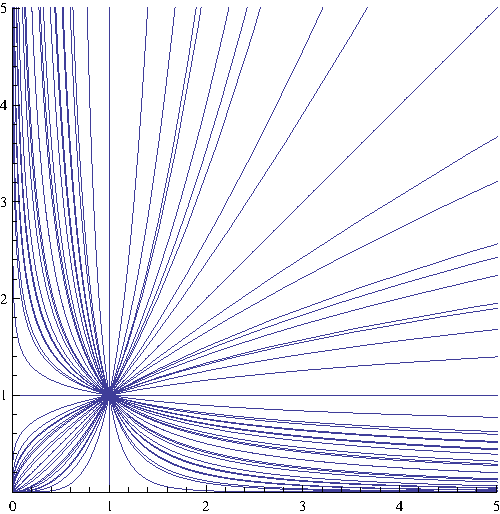
\includegraphics[width=2in]{03-Patterns/support/logspace-picture}

	\item The 3rd and 4th axioms for scalar multiplication fail. 
%	(M1) $k[(a,b)+(c,d)] = k(a+c,b+d) = (2k(a+c),2k(b+d)) = (2ka+2kc,2kb+2kd) = (2ka,2kb)+(2kc,2kd)=k(a,b)+k(c,d)$.
%	(M2) $(j+k)(a,b) = (2(j+k)a,2(j+k)b) = (2ja + 2ka,2jb+2kb) = (2ja,2jb)+(2ka,2kb) = j(a,b)+k(a,b)$.
	(M3) $j(k(a,b)) = j(2ka,2kb)=(2j2ka,2j2kb)=jk(2a,2b)$ instead of $jk(a,b)$.
	(M4) $1(a,b) = (2a,2b)\neq (a,b)$.
	
	
	\item
\begin{enumerate}
	\item 
	Distribution across scalar multiplication fails:  
	$(j+k)(a,b) = (a,(j+k)b) = (a,jb+kb)$ whereas $j(a,b)+k(a,b) = (a,jb)+(a,kb) = (2a,(j+k)b)$ 
	(notice that $a$ is doubled if we multiply first before adding).
	\item  
	Vector addition is not commutative. $(a,b)+(c,d) = (a+c,b)$ while $(c,d)+(a,b) = (a+c,d)$ 
	(the second components are not the same, $b\neq d$.
\end{enumerate}


	\item 
\begin{enumerate}
	\item  Distribution across scalar multiplication fails.
	(M2) $(j+k)(a,b) = ((j+k)^2a,(j+k)b)$ whereas $j(a,b)+k(a,b) = (j^2a,jb)+(k^2a,b) = ((j^2+k^2)a,(j+k)b)$, and $j^2+k^2\neq (j+k)^2$.
	\item  
	Vector addition is not commutative. $(a,b)+(c,d) = (a,d)$ while $(c,d)+(a,b) = (c,b)$.
	
\end{enumerate}


\end{enumerate}



\item \textbf{Vector Subspaces:} 
See chapter 4 problems 13-15, 45-46. Complete at least 13, 15, 46.

\begin{enumerate}
	\item 
		\begin{enumerate}
			\item Yes.  It contains zero, the sum of any two vectors on the $y$ axis is on the $y$ axis, and any scalar multiple of a vector on the $y$ axis is still on the $y$ axis.  The span of $(0,1)$ is the $y$ axis.
			\item No. The zero vector is not on the positive $x$ axis.
			\item No. You cannot times vectors by negative scalars, so it's not closed under scalar multiplication.
			\item Yes. It is the span of $(1,3)$. Lines through the origin are vector subspaces.
			\item No. The line does not contain the zero vector.  It doesn't pass through the origin.
			\item No. It does contain the origin, and is closed under scalar multiplication, but not under vector addition.  The sum $(1,0)+(0,1)=(1,1)$ is not on either axis.
			\item No. Not closed under scalar multiplication. The product $4(1/2,0) = (2,0)$ is not in the set.
		\end{enumerate}


	\item Use theorem \ref{thm subspace iff closed}.
	(1) The zero function is continuous, so zero is in the set. 
	(2) The sum of two continuous functions is a continuous function, so the set is closed under addition.
	(3) A constant times a continuous function is still continuous, so the set is closed under scalar multiplication.
	
	\item Use theorem \ref{thm subspace iff closed}.
	(1) The zero function is a polynomial, so zero is in the set. 
	(2) The sum of two polynomials is a polynomial, so the set is closed under addition.
	(3) A constant times a polynomial is a polynomial, so the set is closed under scalar multiplication.
	
	
	\item 
\begin{enumerate}
	\item 
	(1) The zero function is said to be in the set, so zero is in the set. 
	(2) The sum of two polynomials of degree three must be a polynomial of degree 3 or less, so the set is closed under addition.
	(3) Multiplying a polynomial by a nonzero constant does not change the degree, so the set is closed under scalar multiplication.

	\item The span of the polynomials $\{1,x,x^2,x^3\}$ is $P_3(x)$.  
\end{enumerate}

	\item Let $V$ be the set of 3 by 3 upper triangular matrices.  Show that $V$ is a subspace of the vector space $M_{33}$ of 3 by 3 matrices in 2 ways:
\begin{enumerate}
	\item 
	(1) The zero matrix is upper triangular. 
	(2) The sum of two upper triangular matrices is upper triangular, so the set is closed under addition.
	(3) Multiplying an upper triangular matrix by a constant gives an upper triangular matrix, so the set is closed under scalar multiplication.

	\item 
	The span of 
	$\begin{bmatrix}
	1&0&0\\
	0&0&0\\
	0&0&0
	\end{bmatrix}$,
	$\begin{bmatrix}
	0&1&0\\
	0&0&0\\
	0&0&0
	\end{bmatrix}$,
	$\begin{bmatrix}
	0&0&1\\
	0&0&0\\
	0&0&0
	\end{bmatrix}$,
	$\begin{bmatrix}
	0&0&0\\
	0&1&0\\
	0&0&0
	\end{bmatrix}$,
	$\begin{bmatrix}
	0&0&0\\
	0&0&1\\
	0&0&0
	\end{bmatrix}$,
	$\begin{bmatrix}
	0&0&0\\
	0&0&0\\
	0&0&1
	\end{bmatrix}$
	is the set of upper triangular matrices
  $\begin{bmatrix}
	a&b&c\\
	0&d&e\\
	0&0&f
	\end{bmatrix}$.

	
\end{enumerate}
	\item 
		\begin{enumerate}
			\item 
			Yes. Zero is a symmetric matrix. The sum of two symmetric matrices is symmetric. A constant times a symmetric matrix is symmetric.  Alternatively, the symmetric matrices 
	$\begin{bmatrix}
	a&b\\
	b&c
	\end{bmatrix}$
are spanned by 
	$\begin{bmatrix}
	1&0\\
	0&0
	\end{bmatrix}$
,
	$\begin{bmatrix}
	0&0\\
	0&1
	\end{bmatrix}$
, 
	$\begin{bmatrix}
	0&1\\
	1&0
	\end{bmatrix}$, and hence are a subspace of $M_22$.
			\item	No. The zero matrix is not invertible. 
			\item Yes. Similar to the previous problem related to 3 by 3 matrices.
		\end{enumerate}

	\item 
		\begin{enumerate}
			\item No. The zero polynomial does not have degree 2.
			\item No. The sum of two degree 2 polynomials may be lower in degree.  For example $(x^2) + (x-x^2) = x$. So this set is not closed under addition.
			\item Yes. It is spanned by $\{1,x,x^2\}$
			\item No. Similar to part (b).
		\end{enumerate}

\end{enumerate}




\item \textbf{Spans:} \label{span solutions} \hypertarget{span solutions target}{\hyperlink{span problems target}{(problems link)}}

\begin{enumerate}
	\item 
All but the third have the same row space. The rref of these matrices has the same nonzero rows.


	\item 
All but the third have the same column space. The rref of the transpose of each matrix has the same nonzero rows.

	\item 
		\begin{enumerate}
			\item Yes. The rref is the identity.
			\item No. Only 2 independent columns. Column 3 has coordinates $(3,-1)$.
			\item No. You need at least 3 vectors to span $P_2(x)$.
			\item Yes. There are 3 independent vectors.  The 4th column has coordinates $(1,-1,2)$.
			\item No. Only 2 independent vectors. The coordinates of column 3 are $(1,-1)$, column 4 $(1,2)$.
		\end{enumerate}

	\item 
		\begin{enumerate}
			\item No. You need at least 4 vectors.
			\item Yes.
			\item No. The third polynomial is the sum of the first 2.  There are only 3 independent vectors. 
		\end{enumerate}

	\item 
		\begin{enumerate}
\item 
Yes.

\item 
No.

\item 
No.

\item 
Yes.

		\end{enumerate}
		
\item \textbf{Basis and Dimension:} 
		
\end{enumerate}












\end{enumerate}
\end{multicols}


